% !TeX root = ../thuthesis-example.tex

\chapter{绪论}

\section{研究背景}

随着时代的发展,现阶段,随着城市里的流动车辆数量的不断攀升,给城市的交通带来的负担也日益沉重。根据最新的数据,目前我国的汽车总数已经突破3亿辆,近年来的年均增长率超过2000万辆,而且,每千户家庭的汽车数也已经突破225辆,平均到每百户当中便有60辆汽车。 在当下社会中,人们都过着快节奏的生活,对交通的便捷性需求自然日益增长。越来越多的人会选择出租车或网约车出行;出租车,网约车有着针对性强,更为便捷,流动基数更多等特点,也切实的便捷了人们的出行 。

车联网技术属于物联网技术的范畴,是互联网、电子、汽车等产业融合创新的产物,其旨在通过实现车辆之间的相互通信,最终构建安全高效智能的交通体系 。为了确保车联网的高度稳定,我们必须采取措施来确保它的安全。对此,区块链所具有的去中心化、时序数据、集体维护、可编程和安全可信的特点,使得人们相信其可有效服务于车联网的应用当中 。将区块链技术应用于车联网中,使用区块链技术来构建车辆与路测节点间的特殊自组网,进行车辆间或车辆与路侧节点间的数据交互。通过采取区块链技术,我们能够在车联网中实现更加透明、安全的交易,从而消除中央控制,构建一个更加可信任、无需中央控制的数字资产,从而实现共享经济的发展 。

在出租车调度系统中应用该技术可以消除中介,允许乘客与司机的直接交流与交易,能够为双方提供更为可信的验证,降低信任成本。在网络出租车服务中使用区块链技术有助于参与的所有利益相关方关系更加紧密 。

\section{相关技术调研}

\subsection{区块链概述}

在2008年,一位自称中本聪的人提出了区块链技术 (Blockchain technology,简称BT)。通过使用区块链技术,我们可以建立一个完整、可追溯、可扩展、可信任的网络。区块链利用块链式的数据结构来验证与存储数据,其通过使用共识算法、加密算法、智能合约编程等技术,实现对数据进行安全的访存、传输以及维护,从而实现对信息的有效管理,是一种全新的分布式基础架构与计算范式 。

区块链可以创建无法篡改且端到端加密的记录,用区块链技术所串接的分布式账本能让两方有效纪录交易,且可永久查验此交易,有助于防止欺诈和未经授权的活动。此外,区块链有更大的透明度:由于区块链使用分布式账本,导致交易和数据在多个位置采取完全相同的方式进行记录。区块链技术的核心优势在于它的去中心化特性,即所有拥有访问权限的网络参与者都可以共享相同的信息,从而保证了信息的完全透明度。此外,它的去中心化特性使得每个节点都可以独立地操作,无需受到任何外部干扰,从而提升了系统的可靠性和安全性 。


\subsection{区域索引的树状区块链}

将传统的区块链应用到出租车调度系统中的一个很大的弊端是,传统区块链在面对数量庞大的节点时,因为节点全在一条链上,其查询效率必然会降低;此外,传统区块链结构不能很好地支持对发生在特定区域的事务的查询:用户需要回溯链结构上的所有事务,然后匹配交易发生的位置  。为满足车联网所需的性能要求,大幅度提高地理区块链的区域搜索速度,项目决定用“树状区块链”来代替传统区块链。

在实现树状区块链之前,首先实现了支持区域索引的区块链,该区块链可以基于地理位置信息索引到对应的交易 。之后,在区域索引区块链的基础上,实验室逐步完成了现有的支持区域索引的树状区块链。

如图\ref{fig:树状区块链示意图}所示,树状区块链按照Geohash编码方式划分树状结构,根据不同长度的Geohash编码表示父链与子链关系,文献 说明以Geohash为基础的空间索引算法具有对海量地理数据的高性能查询能力。不同于传统区块链的结构单一,树状区块链结构中的区块根据其作用不同可以划分为创世块(Genesis Block),分支区块(Branch Block)和普通区块(Common Block)三类。

\begin{itemize}
    \item 其中创世块是所有区块的根节点,所有的区块链都有相同的创世块Gensis,然后根据Geohash范围划分不同的区域子链。
    \item 分支区块以Geohash作为索引,是指定分支的第一个区块,只维护直接下层区域的索引信息,不记录交易信息。分支区块由于具备指向同层级前一个分支区块的平行链指针使得原有单链结构成为树状多链构。
    \item 普通区块则基本与传统区块相同。
\end{itemize}

\begin{figure}
	\centering
	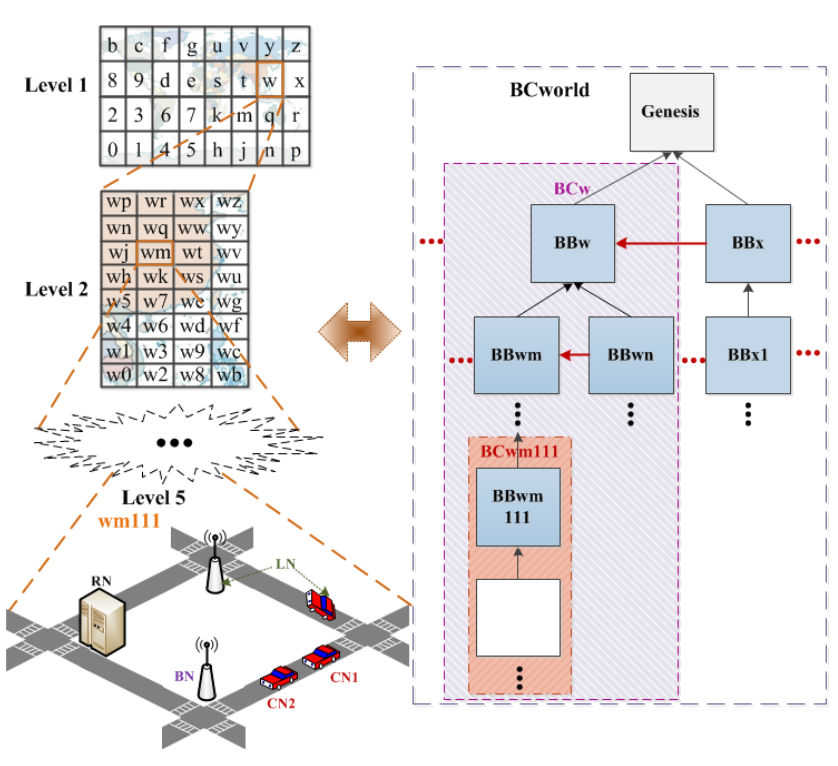
\includegraphics[width=\textwidth]{figures/树状区块链示意图.png}
	\caption{树状区块链示意图}
	\label{fig:树状区块链示意图}
\end{figure}

图\ref{fig:树状区块链内部结构属性示意图}中是树状区块链的内部结构属性示意图,展示了区块链的存储的各种属性,以太坊的结构包括三种查找树:收据查找树、地理状态查找树和交易查找树。除此之外,还添加了一个区域状态查找树来快速查询与分层地理位置相关的数据,以及一个帐户位置查找树来支持查询每辆车的历史交易位置。

\begin{figure}
	\centering
	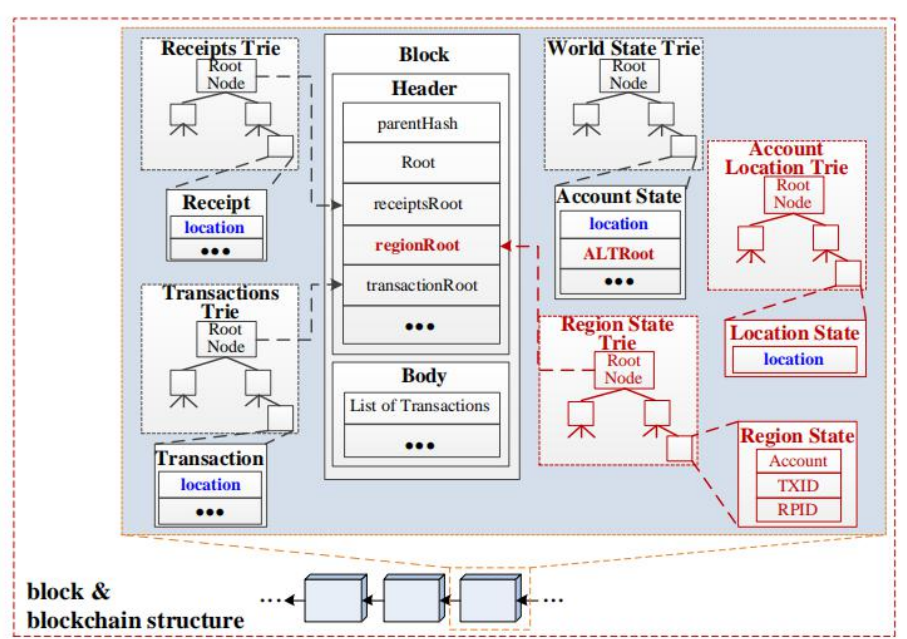
\includegraphics[width=\textwidth]{figures/树状区块链内部结构属性示意图.png}
	\caption{树状区块链内部结构属性示意图}
	\label{fig:树状区块链内部结构属性示意图}
\end{figure}

在现有的工作中,树状区块链在区域查询时可以对各种节点的各种属性进行高速索引,做到既有传统区块链所具有的安全性优势,同时也可以提高区块链的工作效率。但是,目前的工作仍有改善的空间,当前工作针对区域中的搜索可以高效完成,但当节点的地理位置发生较大移动时,此时必须要考虑将节点进行跨链移动,维持多链间的信息同步。简而言之,为使得树状区块链适配更广的适用范围,同时保持工作效率,需要基于现有的出租车调度系统,在其上实现树状区块链的跨链操作。

\subsection{智能合约}

区块链智能合约最早可以追溯到1994年,由Nick Szabo提出 。但真正受到广泛关注和应用是在比特币出现后。智能合约是一种基于区块链技术的自动化数据处理工具,它可以在不受任何第三方干预的情况下实现交易流程。在以太坊中,智能合约还具备信息系统和区块链之间接口的作用 。

智能合约的主要特点包括:
\begin{itemize}
    \item 自动执行:智能合约根据设定的条件和规则自动执行,并在执行完成后更新链上状态。
    \item 去中心化管理:智能合约不需要中心化机构来控制,而是通过代码规则和全网节点来实现管理。
    \item 不可篡改:智能合约一旦被写入区块链,就不能被篡改或删除。
    \item 信任机制:智能合约建立在去中心化的信任机制上,通过全网节点验证执行结果的真实性和正确性 。
\end{itemize}

智能合约的应用如今日益广泛,其可用于处理复杂的金融合约、物流、医疗和电子商务等领域,提高交易效率、降低成本和减少纠纷。 

\section{本文研究内容及贡献}

本文的内容结构如下:文章分为六章:

第一章首先介绍了基于树状区块链的出租车调度系统的应用背景与意义,之后介绍了相关技术的调研情况,最后总结了本文的研究内容及贡献。

第二章则主要针对树状区块链的部分功能实现做了说明,在源码仓库中增添了相应的注释说明。

第三章介绍了基于实验室以往工作而做的区域索引的树状区块链应用于出租车调度系统的复现实验的实验过程。

第四章介绍了对树状区块链应用于出租车调度系统的性能测试实验,验证多子链并行运行的性能负载情况。

第五章介绍了树状区块链的跨链资产转移功能。设计实验验证了树状区块链的跨子链资产转移功能的正确性,并测试了其性能。

第六章,在以上工作的基础之上,本文尝试对现有的出租车调度系统进行跨链交易的改进。现有的出租车调度系统仅支持一个子链内部的交易,针对乘客与车辆分处不同区域的实际应用场景,本文尝试对现有的出租车调度系统进行改进使其支持跨链的交易操作,并最终给出了一个简易的能够实现跨链交易的调度过程,设计实验验证了实现的正确性。


